\chapter{Modelos de machine learning}
\label{cap:modelos}

El procesamiento facial de SmartGate se dividió en tres etapas, cada una orientada a resolver un problema diferente. En primer lugar, YuNet localiza el rostro dentro de la imagen y obtiene la información necesaria para prepararlo. Luego, MiniFASNetV2 evalúa si la muestra presenta características correspondientes a un rostro real o a un intento de suplantación. Finalmente, SFace genera una representación del rostro que permite compararlo con los usuarios registrados.

Esta separación permite utilizar un modelo especializado para cada función y evitar que las etapas de mayor costo se ejecuten sobre imágenes que no resulten adecuadas. Utilizar menos modelos implicaría eliminar alguna de las verificaciones necesarias para la autenticación, mientras que incorporar nuevas redes sin una función diferenciada aumentaría el tiempo de procesamiento y la complejidad de la decisión.

\section{YuNet: detección facial}

\subsection{Elección del modelo}

Se seleccionó YuNet como detector facial de SmartGate debido a que permite localizar rostros mediante una arquitectura compacta y obtener, en una misma inferencia, la información necesaria para preparar las muestras utilizadas posteriormente. Al encontrarse al comienzo del pipeline, esta etapa debe ejecutarse sobre las imágenes provenientes de la cámara antes de conocer si contienen un rostro válido, por lo que resulta conveniente que el procesamiento requerido sea reducido.

El bajo costo computacional de YuNet responde a un diseño orientado a dispositivos con recursos limitados. Su arquitectura combina una red pequeña de extracción de características con una estructura simplificada para integrar información de diferentes escalas. Estas decisiones reducen la cantidad de parámetros que deben almacenarse y el trabajo necesario para procesar cada imagen. En SmartGate, esto favorece la ejecución repetida del detector y permite reservar recursos para las etapas posteriores de verificación de autenticidad y reconocimiento facial. La extracción y combinación de características se explican en el apartado de funcionamiento.

Otro motivo de elección es que YuNet proporciona tanto la ubicación del rostro como los puntos de referencia necesarios para su posterior alineamiento. Disponer de ambas salidas en una misma inferencia evita incorporar un modelo adicional dedicado exclusivamente a localizar estos puntos y simplifica la preparación de las muestras.

La utilización de un detector independiente resulta necesaria porque MiniFASNetV2 y SFace trabajan sobre regiones faciales y no tienen como objetivo buscar personas dentro de una escena completa. YuNet cubre esta necesidad y permite que cada modelo posterior se concentre en su tarea específica.

\subsection{Funcionamiento del modelo}

El flujo comienza con una imagen proveniente de la cámara, que se entrega como entrada a YuNet. Su red convolucional aplica filtros aprendidos durante el entrenamiento para extraer características útiles para la detección facial. Este proceso genera mapas de características con distintas resoluciones espaciales, que representan la información de la imagen a diferentes escalas.

A continuación, una estructura simplificada de pirámide de características combina información de distintos niveles de la red. Esto permite aprovechar tanto detalles espaciales como patrones más generales y facilita la detección de rostros de diferentes tamaños. La extracción y la combinación de características forman parte de una misma inferencia.

A partir de estas representaciones, el modelo genera detecciones candidatas. Cada una contiene un cuadro delimitador (\textit{bounding box}), una puntuación de confianza y cinco puntos de referencia faciales (\textit{landmarks}), correspondientes a los dos ojos, la nariz y las dos comisuras de la boca. El cuadro indica la ubicación y el tamaño del rostro, mientras que la confianza permite valorar la detección. Esta puntuación no determina la identidad de la persona ni la autenticidad del rostro.

Las predicciones pasan luego por una etapa de posprocesamiento. Primero se descartan las candidatas cuya confianza se encuentra por debajo del umbral configurado. Después se aplica supresión de no máximos (\textit{Non-Maximum Suppression}, NMS), que prioriza las detecciones de mayor confianza y elimina aquellas que se superponen excesivamente con ellas. De esta manera, se reducen las detecciones repetidas sobre un mismo rostro.

El detector devuelve las detecciones conservadas junto con sus cuadros delimitadores, puntuaciones de confianza y puntos faciales. Si ninguna candidata supera el filtrado, el resultado no contiene rostros detectados.

Las etapas posteriores del pipeline utilizan esta información para preparar las muestras. El cuadro delimitador permite localizar la región facial que se debe recortar, mientras que los puntos de referencia permiten calcular el alineamiento previo al reconocimiento. Este último ajusta la posición, la escala y la inclinación del rostro en el plano de la imagen. El recorte y el alineamiento son operaciones posteriores a la detección realizada por YuNet.

\subsection{Diagrama de flujo del modelo}

\begin{figure}[H]
    \centering
    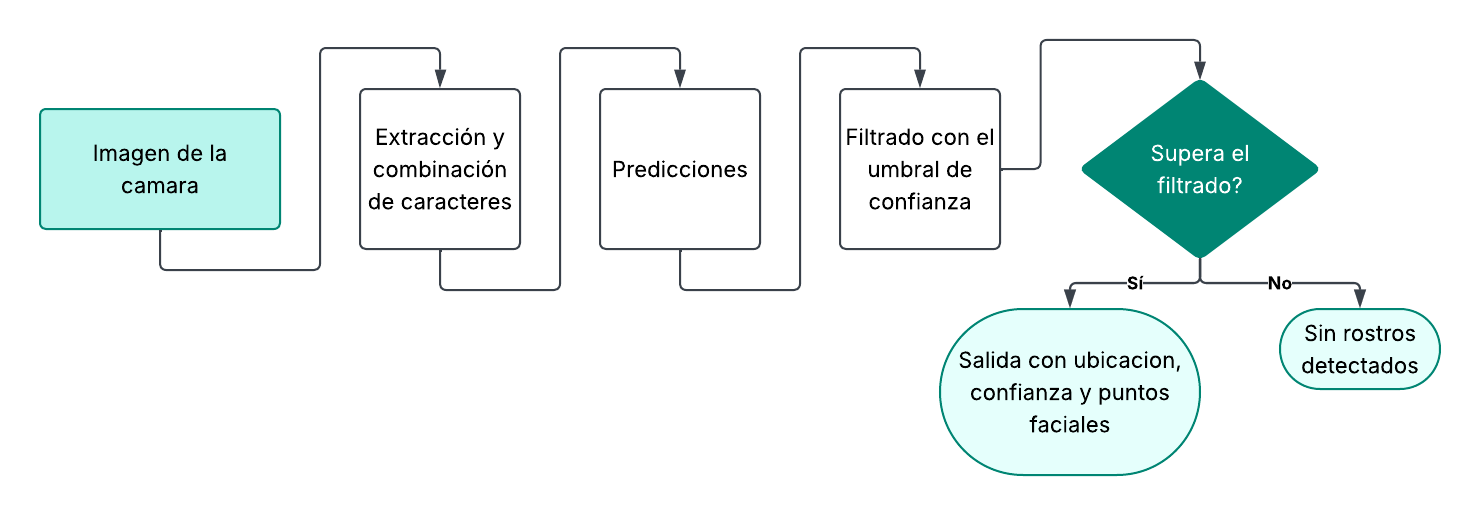
\includegraphics[width=\textwidth]{Imagenes/flujo_yunet.png}
    \caption{Diagrama de flujo de YuNet.}
    \label{fig:flujo-yunet}
\end{figure}

\section{MiniFASNetV2: antispoofing}

\subsection{Elección del modelo}

Se seleccionó MiniFASNetV2 para la detección de intentos de suplantación debido a que la identificación de una persona por sí sola no permite determinar si el rostro observado proviene de una persona físicamente presente. Una fotografía impresa o una imagen mostrada en una pantalla puede conservar suficientes características de identidad para ser reconocida. Por este motivo, antes de utilizar el resultado de SFace para autorizar un acceso se incorpora una etapa independiente de anti-spoofing.

MiniFASNetV2 pertenece a una familia de redes diseñadas específicamente para esta tarea y desarrolladas a partir de una arquitectura basada en MobileFaceNet. Su tamaño reducido responde a la aplicación de poda de canales, que disminuye la cantidad de información intermedia que debe procesar la red y, con ello, sus parámetros y operaciones. Además, utiliza bloques que combinan convoluciones por canal y convoluciones puntuales, permitiendo extraer características con un costo menor que el de convoluciones convencionales equivalentes. El funcionamiento de estos bloques se explica en el apartado siguiente.

Estas características resultan convenientes para SmartGate porque permiten agregar una evaluación de autenticidad sin introducir una red de gran tamaño en el pipeline. Esto favorece el procesamiento frecuente de muestras faciales y deja recursos disponibles para la detección y el reconocimiento. Asimismo, el modelo analiza imágenes sin requerir que la persona complete una secuencia de acciones, lo que permite incorporar la comprobación al flujo de acceso sin solicitar gestos adicionales.

MiniFASNetV2 se utiliza como único modelo para esta etapa porque agrega una comprobación que ni YuNet ni SFace realizan. Eliminarlo permitiría que una muestra correctamente detectada e identificada avanzara sin evaluar su autenticidad, mientras que utilizar varios clasificadores de anti-spoofing obligaría a realizar inferencias adicionales y combinar sus resultados. Su elección permite incorporar esta segunda condición de seguridad manteniendo una etapa específicamente dedicada a detectar intentos de suplantación.

La separación respecto del reconocimiento también permite ajustar el criterio de aceptación del anti-spoofing sin modificar la comparación de identidades realizada por SFace.

\subsection{Funcionamiento del modelo}

El flujo comienza con la imagen de la cámara y la ubicación del rostro obtenida mediante YuNet. A partir de esta información se prepara un recorte facial, conservando el contexto alrededor del rostro que requiera la versión del modelo utilizada. Luego se ajusta el recorte al tamaño de entrada correspondiente y se convierte en un tensor, es decir, una representación numérica organizada que la red puede procesar. Esta preparación debe respetar las condiciones de entrada previstas durante el entrenamiento.

La muestra atraviesa una serie de bloques convolucionales que extraen características visuales aprendidas para distinguir rostros reales de representaciones utilizadas como ataque. Dentro de estos bloques, las convoluciones por canal (\textit{depthwise}) procesan por separado cada canal de características, mientras que las convoluciones puntuales de $1 \times 1$ combinan información entre canales. Esta separación reduce el cálculo necesario para transformar las representaciones internas.

La red también incorpora conexiones residuales, que suman la entrada de determinados bloques a su salida y facilitan la propagación de información. A medida que avanza el procesamiento, se reduce la resolución espacial de los mapas de características hasta obtener una representación compacta de la muestra.

Esta representación se entrega a una capa de clasificación, que produce una puntuación sin normalizar, denominada \textit{logit}, para cada clase considerada durante el entrenamiento. En la implementación de referencia, estas puntuaciones se transforman mediante la función \textit{softmax}, obteniendo valores entre cero y uno cuya suma es uno. Estos valores expresan la preferencia relativa del clasificador por cada clase.

La interpretación de la salida permite distinguir la clase correspondiente a una muestra real de las asociadas a ataques. Sobre estas puntuaciones, la aplicación aplica su criterio de aceptación del anti-spoofing. La clasificación y el criterio de aceptación constituyen pasos diferentes: la red produce puntuaciones y la lógica del sistema determina si resultan suficientes para aceptar la muestra.

Si el criterio no se cumple, la muestra no supera esta comprobación. Si se cumple, queda satisfecha la condición de anti-spoofing, cuyo resultado se combina con la evaluación de identidad realizada mediante SFace. Por lo tanto, la salida de MiniFASNetV2 aporta una estimación de autenticidad y no constituye, por sí sola, una autorización de acceso.

\subsection{Diagrama de flujo del modelo}

\begin{figure}[H]
    \centering
    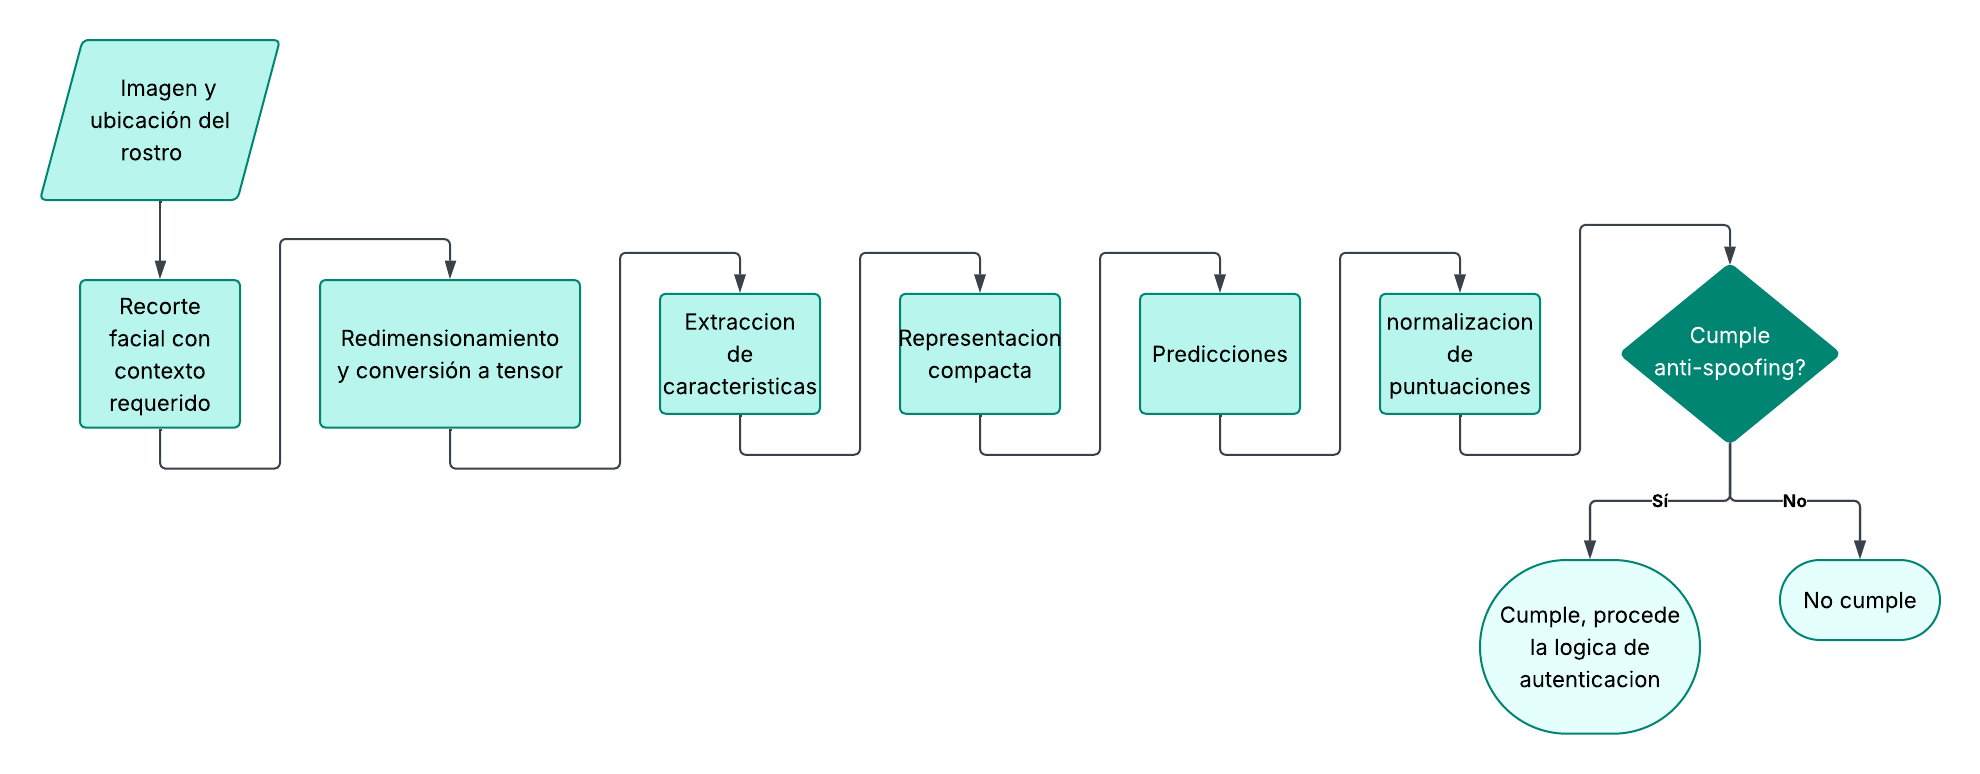
\includegraphics[width=\textwidth]{Imagenes/flujo_minifasnet.png}
    \caption{Diagrama de flujo de MiniFASNetV2.}
    \label{fig:flujo-minifasnet}
\end{figure}

\section{SFace: reconocimiento facial}

\subsection{Elección del modelo}

Se seleccionó SFace como modelo de reconocimiento facial de SmartGate para determinar la identidad del rostro que superó las etapas anteriores. A diferencia de un clasificador convencional, el modelo no genera directamente una clase correspondiente a cada usuario, sino una representación numérica de las características de la cara denominada \textit{embedding}.

Esta forma de representar los rostros resulta conveniente porque separa el modelo de reconocimiento de la cantidad concreta de usuarios registrados. Incorporar una nueva persona requiere obtener y almacenar su representación facial, en lugar de crear una nueva salida y volver a entrenar toda la red. Esto simplifica la administración de usuarios y permite actualizar el conjunto de personas autorizadas sin modificar el modelo.

Otro motivo de elección es que el entrenamiento mediante SFace busca obtener representaciones que permitan distinguir identidades, moderando la influencia de muestras problemáticas para reducir el sobreajuste a errores presentes en los datos de entrenamiento. Esta característica favorece la obtención de representaciones útiles para la comparación facial. La relación entre este entrenamiento y los vectores obtenidos se explica en el apartado de funcionamiento.

Además, la implementación disponible en OpenCV permite integrar la extracción de características y su comparación con el alineamiento basado en los cinco puntos faciales proporcionados por YuNet. Esta compatibilidad simplifica la conexión entre la detección y el reconocimiento, aprovechando información que ya se obtiene en una etapa anterior.

SFace constituye la última de las tres redes porque responde una pregunta que las etapas anteriores no resuelven. YuNet determina dónde se encuentra el rostro y MiniFASNetV2 evalúa su autenticidad, pero ninguno establece a quién pertenece. La combinación de los tres modelos permite así obtener de forma secuencial la localización, autenticidad e identidad necesarias para que la lógica de SmartGate tome la decisión final de acceso.

\subsection{Funcionamiento del modelo}

El flujo de reconocimiento comienza con el rostro que superó la comprobación de anti-spoofing. A partir de los puntos faciales obtenidos mediante YuNet, se realiza el alineamiento y el recorte de la imagen. Este procedimiento ajusta la posición, la escala y la inclinación del rostro en el plano de la imagen para que las muestras presenten una disposición comparable antes de ingresar a la red.

La imagen preparada se convierte al formato numérico de entrada requerido por el modelo. Esta conversión a tensor organiza los valores de los píxeles; todavía no constituye la generación del embedding. Posteriormente, la red convolucional procesa esos valores y extrae progresivamente características hasta producir un vector de longitud fija que representa información relevante para distinguir identidades.

En la versión distribuida por OpenCV, la red utilizada es MobileFaceNet, entrenada mediante la función de pérdida SFace. Durante el entrenamiento, esta función regula la aproximación de representaciones de una misma identidad y la separación de identidades diferentes. Para ello utiliza funciones sigmoides que moderan la contribución de las muestras al aprendizaje, buscando reducir el sobreajuste a datos problemáticos. Este procedimiento pertenece al entrenamiento previo y no se repite cada vez que SmartGate analiza un rostro.

Durante el uso del sistema, la salida de la red es el embedding de la muestra. La identificación se obtiene al compararlo con las representaciones almacenadas para los usuarios autorizados. Las muestras de registro deben prepararse y procesarse con el mismo modelo para que sus vectores sean comparables.

La comparación se realiza mediante una métrica. Con una métrica de similitud, los valores más altos indican una mayor semejanza; con una distancia, la mayor semejanza corresponde a valores más bajos. A partir de estas comparaciones se selecciona la mejor coincidencia y se comprueba si cumple el umbral de reconocimiento establecido.

Si la mejor coincidencia no cumple el umbral, la muestra se considera no reconocida, aunque exista un usuario cuyo vector sea el más cercano. Si lo cumple, se obtiene la identidad asociada a esa representación. Este resultado se entrega a la lógica de SmartGate, que lo utiliza junto con las comprobaciones anteriores y las condiciones de autorización para decidir el acceso.

\subsection{Diagrama de flujo del modelo}

\begin{figure}[H]
    \centering
    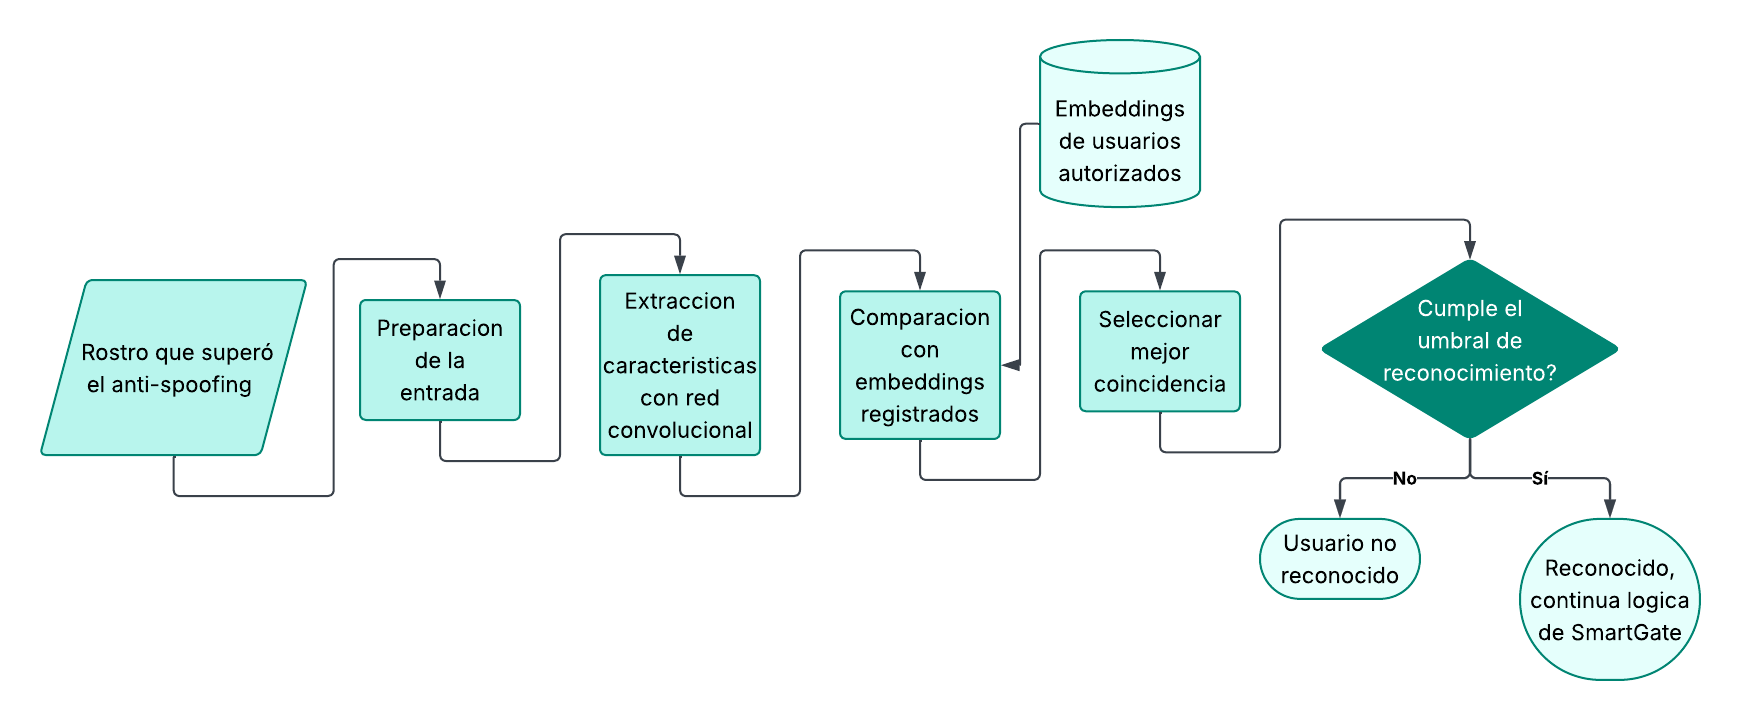
\includegraphics[width=\textwidth]{Imagenes/flujo_sface.png}
    \caption{Diagrama de flujo de SFace.}
    \label{fig:flujo-sface}
\end{figure}
